% ============================================================================
\section{Neural end-to-end TTS}
% ============================================================================

\begin{frame}[allowframebreaks]{2016--2021 Era: The Neural Revolution (WaveNet)}
    \begin{itemize}
        \item Deep generative model for raw audio
        \item Autoregressive: predicts next sample given previous samples
        \item High-quality, natural-sounding speech
        \item Equation:
        \[
            p(x) = \prod_{t=1}^{T} p(x_t | x_{1}, ..., x_{t-1})
        \]
        \item Computationally expensive for real-time use
    \end{itemize}
    \begin{center}
        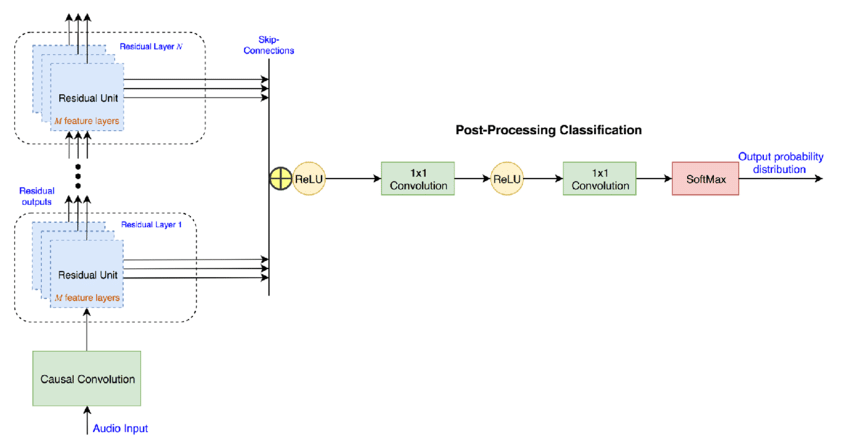
\includegraphics[width=\textwidth,height=0.9\textheight,keepaspectratio]{images/audio-nlp/wavenet_architecture.png}
    \slideimgsource{van den Oord et al., WaveNet, after \href{https://deepmind.google/discover/blog/wavenet-a-generative-model-for-raw-audio/}{DeepMind}.}
    \end{center}
\end{frame}

\begin{frame}{2016--2021 Era: Neural vocoders (WaveNet and beyond)}
  \begin{itemize}\footnotesize
    \item Mel-spectrograms show how frequencies change over time, but must be turned back into sound waveforms.
    \item The Griffin-Lim algorithm was an early method for this, but the quality was limited.
    \item Neural vocoders like WaveNet can reach human-level speech quality.
    \item WaveNet generates raw audio samples one by one, at up to 24,000 times per second.
    \item It uses dilated causal convolutions, so it can “see” a lot of context efficiently.
    \item WaveNet models the conditional probability of each sample: \[
      p(\mathbf{x} \mid \mathbf{h}) = \prod_{t=1}^{T} p(x_t \mid x_1, \dots, x_{t-1}, \mathbf{h})
    \]
    where $\mathbf{h}$ is the mel-spectrogram.
    \item This approach gives very natural speech, but it is slow to run for real-time use.
  \end{itemize}
\end{frame}

\begin{frame}{2016--2021 Era: End-to-end Neural TTS (Tacotron)}
  \centering
  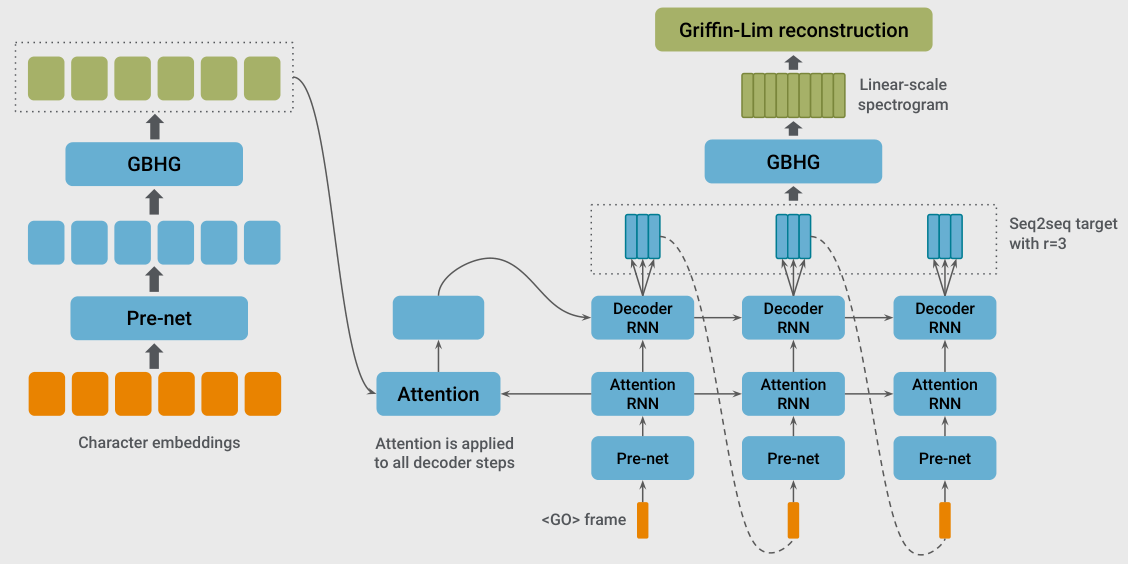
\includegraphics[width=0.98\textwidth,keepaspectratio]{assets/New-Lecture-TTS/cs224s_2024_lec1/slide_31.png}
  \slideimgsource{Tacotron (Wang et al, 2017); Model Architecture. The model takes characters as input and outputs the corresponding raw spectrogram, which is then fed to the Griffin-Lim reconstruction algorithm to synthesize speech.}
\end{frame}


\begin{frame}[allowframebreaks]{Tacotron 2}
    \begin{itemize}
        \item End-to-end TTS system
        \item Pipeline:
        \begin{itemize}
            \item Text $\rightarrow$ Mel-spectrogram (sequence-to-sequence model)
            \item Mel-spectrogram $\rightarrow$ WaveNet/GAN vocoder (audio synthesis)
        \end{itemize}
        \item Improved prosody and pronunciation
        \item Flexible for different voices and languages
    \end{itemize}
    \begin{center}
        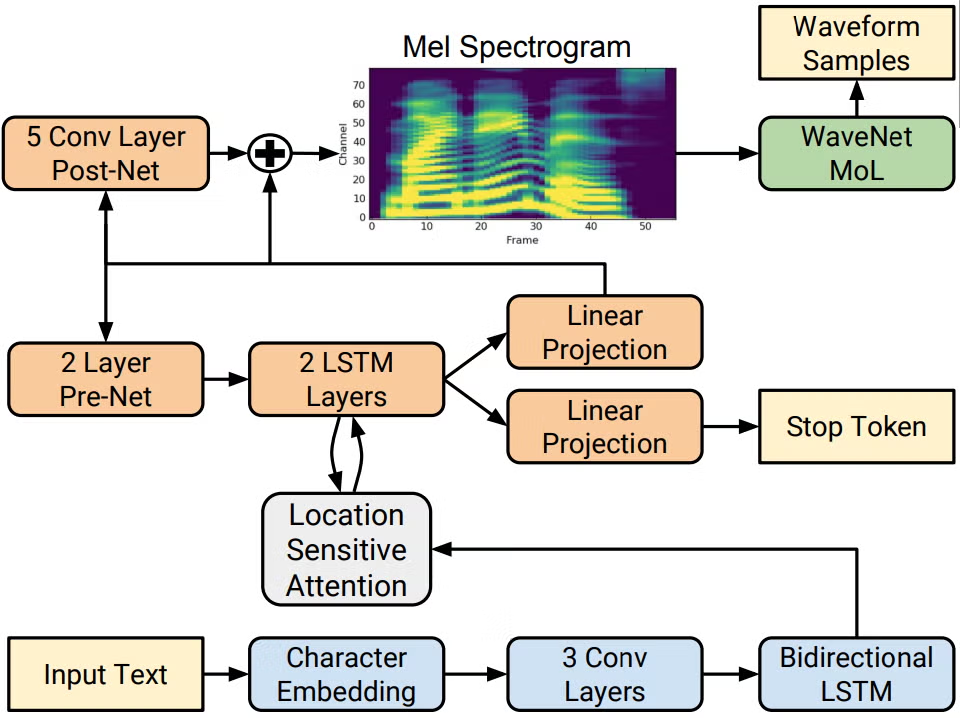
\includegraphics[width=\textwidth,height=0.8\textheight,keepaspectratio]{images/audio-nlp/tacotron2_pipeline.png}
        \slideimgsource{Tacotron 2, after \href{https://arxiv.org/abs/1712.05884}{Shen et al., 2018.}.}
    \end{center}
\end{frame}

% --- Source: Shen et al.\ Tacotron~2 (Works cited 8); WaveNet (Works cited in report) ---

\begin{frame}{Autoregression: the deployment bottleneck}
  \begin{itemize}
    \item Tacotron~2 + WaveNet-class vocoders raised fidelity but blocked low-latency, on-device synthesis.
    \item Motivated \textbf{non-autoregressive (NAR)} acoustic models and fast vocoders (FastSpeech, HiFi-GAN).
  \end{itemize}
\end{frame}

\begin{frame}[allowframebreaks]{2022--present: FastSpeech, HiFi-GAN, Glow-TTS, Diffusion Models}
  \begin{itemize}
      \setlength{\itemsep}{1.5em}
      \item Non-autoregressive models: faster inference
      \item FastSpeech:
      \begin{itemize}
          \item Parallel generation of spectrograms
          \item Duration prediction for alignment
      \end{itemize}
      \item HiFi-GAN:
      \begin{itemize}
          \item GAN-based vocoder
          \item High-fidelity, real-time synthesis
      \end{itemize}
  \framebreak
      \item Glow-TTS:
      \begin{itemize}
          \item Flow-based generative model
          \item Efficient and expressive speech synthesis
      \end{itemize}
      \item Diffusion models:
      \begin{itemize}
          \item Iterative refinement of audio
          \item State-of-the-art naturalness
      \end{itemize}
  \end{itemize}
  \begin{center}
      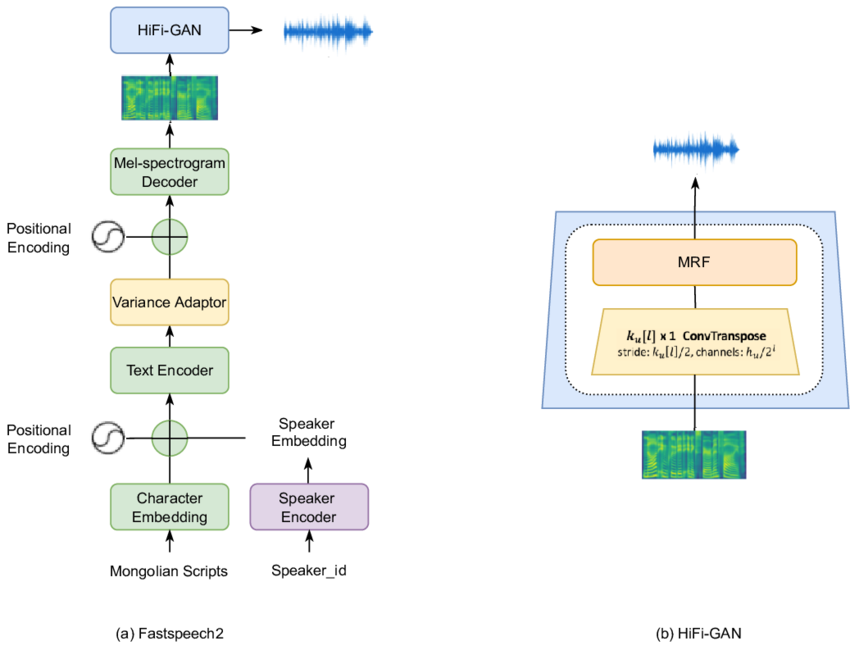
\includegraphics[width=\textwidth,height=0.9\textheight,keepaspectratio]{images/audio-nlp/fastspeech_hifigan.png}
  \end{center}
\end{frame}

% --- Source: Jurafsky SLP3 Ch.16 (Works cited 25); Lecture-12 mel\_filterbanks ---
% \begin{frame}{Mel spectrograms for acoustic modeling}
%   \begin{itemize}
%     \item STFT $\rightarrow$ mel filterbank (40--80 bands) $\rightarrow$ log magnitudes $\Rightarrow$ time $\times$ mel matrix.
%     \item Mel scale matches human pitch perception; log compression stabilizes dynamic range for neural nets.
%     \item Standard target for Tacotron-class models; shared feature family with modern ASR front ends.
%   \end{itemize}
%   \centering
%   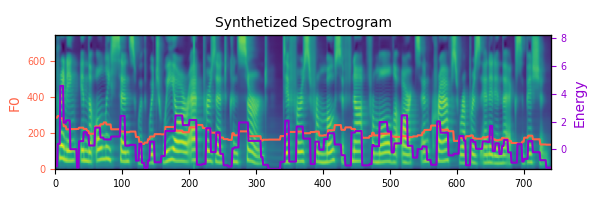
\includegraphics[width=0.90\textwidth,keepaspectratio]{assets/New-Lecture-TTS/tts_mel_spectrogram.png}
%   \slideimgsource{Illustrative log-mel spectrogram (teaching asset); representation family as in Shen et al., Tacotron~2.}
% \end{frame}

% % --- Source: CMU Alan Black / Festvox (Works cited 5--6); TTS Lecture Material Generation Request ---
% \begin{frame}{Linguistic front end (CMU tradition)}
%   \begin{itemize}
%     \item \textbf{Text normalization:} numbers, dates, symbols, abbreviations---most production bugs start here.
%     \item \textbf{G2P:} grapheme-to-phoneme rules, lexicons, or neural G2P for opaque orthographies.
%     \item \textbf{Low-resource voices:} careful data collection (Festvox-style prompts), phonetic coverage, and prosody labels.
%     \item SSML / markup in deployed systems for breaks, emphasis, and speaking rate.
%   \end{itemize}
% \end{frame}
